\section{PyAlarmClock}
Pro usnadnění manipulace s budíkem připojeným přes rozhraní UART z počítače
byla vytvořena knihovna \texttt{PyAlarmClock}. Je to modul jazyka Python
obsahující abstrakce pro práci s budíkem. Programátor vytvářející počítačový
program díky tomu nemusí ani znát konkrétní příkazy prostředí
\texttt{AlarmClockCLI}. Například nastavení data času modulu RTC se provádí
přiřazením objektu \texttt{datetime.datetime} vlastnosti \verb|RTC_time|
objektu \texttt{AlarmClock} bez nutnosti znát vnitřní implementaci, která
využívá příkazu \texttt{st} pro nastavení času a \texttt{sd} pro nastavení
data.

Pro ilustraci konceptu poslouží jeden z ukázkových programů~--
\repopath{src/PyAlarmClock/examples/set_time.py}. V následující ukázce je navíc
odstraněna část zapínající podrobné protokolování všech událostí.
\begin{lstlisting}[language=Python,style=numbers]
#!/usr/bin/env python3

import PyAlarmClock
from datetime import datetime
import time

with PyAlarmClock.SerialAlarmClock('/dev/ttyUSB0') as ac:
    ac.RTC_time = datetime.now()
    time.sleep(1.65)  # RTC is polled every 0.8 seconds
    print(ac.RTC_time)
\end{lstlisting}
Program naváže spojení s budíkem, nastaví čas uložený v RTC na aktuální čas,
počká \SI{1,65}{\second} (aby stihl firmware budíku přečíst novou hodnotu
z RTC) a vypíše do konzole čas přečtený z budíku.
\begin{lstlisting}[style=terminal]
$ ./set_time.py
2022-02-08 19:21:48
$
\end{lstlisting}


\subsection{MQTT adaptér}
Jedním z programů využívajících knihovnu \texttt{PyAlarmClock} je
\repopath{src/PyAlarmClock/cmds/mqtt_bridge.py} (po instalaci balíčku dostupný
jako \shellcmd{ac2mqtt}). Tento program umožňuje vzdálené ovládání budíku
zprávami přenášenými protokolem MQTT. Tímto způsobem lze zajistit ovládání
budíku několika programy současně bez nutnosti sdílet sériový port mezi více
procesy. Komunikace může probíhat nejen mezi více zařízeními ve stejné
počítačové síti, ale i v rámci jednoho serveru (\texttt{localhost}).

Použití adaptéru je velmi jednoduché. Příkazem \verb|ac2mqtt --help|
lze vypsat seznam argumentů, které lze programu předávat.
% nechci sem davat cely usage, protoze bych ho pak treba musel aktualizovat...
Následuje jednoduchý příklad~-- program se připojí k MQTT brokeru na
\texttt{localhost} na výchozím portu 1883 jako uživatel \texttt{DEBUG} s heslem
zadaným interaktivně za běhu programu:
\begin{lstlisting}[style=terminal]
$ ac2mqtt /dev/ttyUSB0 -u DEBUG
Password:
2022-02-08 19:22:39,360 INFO err topic: alarmclock/err
2022-02-08 19:22:39,360 INFO state topic: alarmclock/stat
2022-02-08 19:22:39,360 INFO command topic: alarmclock/cmnd
2022-02-08 19:22:39,361 INFO Connecting to MQTT on localhost:1883
2022-02-08 19:22:42,139 INFO MQTT connected with result code 0

\end{lstlisting}

Pomocí nástrojů ze softwarového balíčku \texttt{mosquitto-clients}
% https://packages.ubuntu.com/focal/mosquitto-clients
můžeme pozorovat, že program při spuštění odešle několik zpráv:
\begin{lstlisting}[style=terminal]
$ mosquitto_sub -v -t alarmclock/#
alarmclock/stat/available online
alarmclock/stat/number_of_alarms 6
\end{lstlisting}
Číslo posílané v topic \topic{alarmclock/stat/number_of_alarms} udává počet
konfigurovatelných časů buzení, které firmware připojeného budíku podporuje
(interně zjišťováno příkazem \texttt{ver}). Zpráva je adaptérem zasílána
s příznakem \texttt{retain}, proto je automaticky zaslána nově příchozímu
subscriberovi.

Zpráva v topic \topic{alarmclock/stat/available} určuje, zda je adaptér
aktivní. Při jeho ukončení či náhodném odpojení je MQTT brokerem do tohoto
topic automaticky zaslána zpráva \texttt{offline}. K tomu je využívána funkce
MQTT \ac{LWT}.

Požadujeme-li, aby budík provedl nějakou akci, pošleme zprávu do příslušného
\texttt{command topic} -- \topic{alarmclock/cmnd/nazev_prikazu}.
Toto je interně řešeno pomocí základních tříd \texttt{AlarmClockMQTT.Entity}
a \texttt{AlarmClockMQTT.Command}, ze kterých dědí třídy reprezentující
jednotlivé komponenty budíku. \texttt{Entity} reprezentuje komponentu mající
nějaký stav, který je možné na vyžádání přečíst
(\foreignlanguage{english}{polling}). \texttt{Command} reprezentuje příkaz,
který je možné spustit MQTT zprávou. Příkazy nemají žádný vlastní stav.
Třídy jednotlivých komponent mohou dědit z obou těchto základních tříd
zároveň~-- například \texttt{Switch} je přepínač, který lze vzdáleně ovládat
a jehož stav je možné i číst.

\begin{lstlisting}[language=Python]
class AlarmClockMQTT:
    """An MQTT adapter for AlarmClock."""

    class Entity:
        """Representation of an AlarmClock attribute with a pollable state."""

        def get_state(self, ac: AlarmClock):
            """Get state of the entity.

            Returns a result that should be published in the entity's
            state_topic.
            """
            raise NotImplementedError()

    class CommandError(Exception):
        """Error raised by a MQTT command handler."""

    class Command:
        """Representation of a MQTT command handler."""

        def do_command(self, ac: AlarmClock, msg: str):
            """Handle reception of msg.

            The return value (if not None) of this function will be published
            in the corresponding state_topic.

            If a tuple is returned, the first value in the tuple is a topic
            under state_topic where the second value should be published.

            If a list is returned, each item will be handled according to
            the above rules.
            """
            raise NotImplementedError()

    class Switch(Entity, Command):
        """A switch that can either be OFF or ON.

        e.g. lamp, inhibit
        """

        def __init__(self, name: str):
            """Initialize a switch.

            name must be a valid name of a AlarmClock attribute.
            """
            self.name = name

        def do_command(self, ac: AlarmClock, msg: str):
            messages = {
                'ON': lambda ac: self.turn_on(ac),
                'OFF': lambda ac: self.turn_off(ac),
                '?': lambda ac: None,  # empty lambda - only stat
                '': lambda ac: None,
            }

            msg = msg.upper()
            if msg in messages:
                messages[msg](ac)
                return self.get_state(ac)
            else:
                raise AlarmClockMQTT.CommandError()

        def turn_on(self, ac: AlarmClock):
            setattr(ac, self.name, True)

        def turn_off(self, ac: AlarmClock):
            setattr(ac, self.name, False)

        def get_state(self, ac: AlarmClock):
            value = getattr(ac, self.name)
            value = 'ON' if value else 'OFF'
            return value
\end{lstlisting}

Instance \texttt{AlarmClockMQTT} má svá asociativní pole
\texttt{ENTITIES} a \texttt{COMMANDS}, ve kterých jsou uloženy jednotlivé
instance entit a příkazů přiřazené ke svému \texttt{topic}.

\begin{lstlisting}[language=Python]
class AlarmClockMQTT:
    # ...

    def __init__(self, config: AlarmClockMQTTConfig):
        # ...
        ambient = self.DimmableLight('ambient')

        self.COMMANDS: Dict[str, AlarmClockMQTT.Command] = {
            'ambient': ambient,
            # ...
        }

        self.ENTITIES: Dict[str, AlarmClockMQTT.Entity] = {
            'ambient': ambient,
            # ...
        }
\end{lstlisting}

Pro všechny entity, které nejsou zároveň příkazem, je implementováno čtení na
vyžádání, které se provádí MQTT zprávou se znakem \texttt{?} v \texttt{payload}
zaslanou do \texttt{topic} \topic{alarmclock/cmnd/nazev_entity}. Odpověď je
zaslána do \topic{alarmclock/stat/nazev_entity}, \texttt{payload} zprávy je
určen konkrétní implementací metody \verb|get_state| v objektu dané entity.
Entity, které jsou zároveň příkazem (nebo čisté příkazy bez vlastního stavu),
musí zprávy s \lstinline[language=Python]!payload = '?'! v případě potřeby
ošetřit ve vlastní implementaci metody \verb|do_command|. Do
\topic{alarmclock/stat/nazev_entity} je poté zaslána hodnota vrácená touto
metodou. Informace o případných chybách jsou zasílány do
\topic{alarmclock/err}.

\begin{lstlisting}[language=Python]
class AlarmClockMQTT:
    # ...

    def _on_message(self, client, userdata, msg):
        if self._config.command_topic in msg.topic:
            command_id = remove_prefix(msg.topic,
                                       f'{self._config.command_topic}/')
            payload = msg.payload.decode('ascii')
            if command_id in self.COMMANDS:
                self._execute_command(client, command_id, payload)
            elif command_id in self.ENTITIES and payload == '?':
                entity_id = command_id
                self._report_state(client, entity_id)
            else:
                text = f'Bad topic for command: {msg.topic}'
                _LOGGER.error(text)
                client.publish(self._config.err_topic, text)

    def _report_state(self, client: mqtt.Client, entity_id: str):
        client.publish(f'{self._config.state_topic}/{entity_id}',
                       self.ENTITIES[entity_id].get_state(self.ac))

    def _execute_command(self, client: mqtt.Client, command_name: str,
                         msg: str):
        try:
            ret = self.COMMANDS[command_name].do_command(self.ac, msg)
            if ret is not None:
                if not isinstance(ret, list):
                    ret = [ret]
                for value in ret:
                    if isinstance(value, tuple):
                        topic, message = value
                        client.publish(f'{self._config.state_topic}/{topic}',
                                       message)
                    else:
                        client.publish(
                                f'{self._config.state_topic}/{command_name}',
                                value
                                )
        except self.CommandError as e:
            # ...
\end{lstlisting}

V následujícím příkladu je demonstrované rozsvícení připojeného světla
\texttt{lamp} vzdáleným MQTT příkazem a následné zhasnutí pomocí rozhraní na
displeji budíku. Pro přehlednost byly přidány prázdné řádky. První zpráva
v druhém bloku je příkaz pro rozsvícení lampy. V odpověď na ni přichází zpráva
v topic \topic{alarmclock/stat/lamp} značící, že byla lampa rozsvícena. Protože
firmware budíku podporuje funkci přidanou z vývojové větve
\texttt{feature/CLI-BEL}, posílá při každé změně stavu hardware na sériový port
netisknutelný ASCII znak BEL (\texttt{0x07}). V reakci na to si adaptér vyžádá
stav všech hardwarových výstupů a odešle příslušné MQTT zprávy. Zpráva o stavu
lampy je proto duplikována, je ale zajištěna zpětná kompatibilita s firmware
bez podpory funkce asynchronní detekce změn stavu hardware.
Díky této funkci je detekováno i vypnutí lampy přímo ovládacími prvky budíku,
které vede k odeslání třetího bloku zpráv.
\begin{lstlisting}[style=terminal]
$ mosquitto_sub -v -t alarmclock/#
alarmclock/stat/available online
alarmclock/stat/number_of_alarms 6

alarmclock/cmnd/lamp ON
alarmclock/stat/lamp ON
alarmclock/stat/lamp ON
alarmclock/stat/inhibit OFF
alarmclock/stat/ambient 0

alarmclock/stat/lamp OFF
alarmclock/stat/inhibit OFF
alarmclock/stat/ambient 0
\end{lstlisting}

Toto rozhraní funguje velmi dobře pro jednoduché entity, jako například výše
zmíněné světlo. Například pro konfiguraci jednotlivých budicích časů by ale
bylo vhodnější využít komunikační protokol, který navazuje přímé spojení mezi
klientem a serverem a páruje odpovědi ke konkretním požadavkům. Takovým
protokolem je například HTTP, ten je ale zase naprosto nevhodný pro entity,
u nichž potřebujeme přijímat asynchronní informace o jejich stavu.

MQTT API je v současné době používáno i pro nastavování budicích časů, ty jsou
pro účely přenosu v textových zprávách serializovány do formátu JSON.
Každému budicímu času odpovídá jeden MQTT topic. Aby klient používajíci API
věděl, kolik budicích časů budík podporuje, je do topic
\topic{alarmclock/stat/number_of_alarms} zasílána zpráva s příznakem
\texttt{retain} obsahující jejich celkový počet.

Přečtení prvního budicího času probíhá následujícím způsobem:
\begin{lstlisting}[style=terminal]
$ mosquitto_pub -t alarmclock/cmnd/alarm -m '0'
\end{lstlisting}

\begin{lstlisting}[style=terminal]
$ mosquitto_sub -v -t alarmclock/#
alarmclock/stat/available online
alarmclock/stat/number_of_alarms 6

alarmclock/cmnd/alarm 0
alarmclock/stat/alarms/alarm0 {"enabled": "OFF", "days_of_week": ["Friday"], "time": {"hours": 12, "minutes": 34}, "snooze": {"time": 1, "count": 1}, "signalization": {"ambient": 120, "lamp": true, "buzzer": 1}}
\end{lstlisting}

Zápis se provádí zasláním JSON objektu do topic odpovídajícího příkazu
\texttt{WriteAlarmCommand}. Číslo zapisovaného času buzení je určeno hodnotou
přiřazenou klíči \texttt{index} v tomto objektu.
\begin{lstlisting}[style=terminal]
$ mosquitto_pub -t alarmclock/cmnd/alarm/write -m '{"index": 0, "enabled": "OFF", "days_of_week": ["Friday"], "time": {"hours": 12, "minutes": 0}, "snooze": {"time": 1, "count": 1}, "signalization": {"ambient": 0, "lamp": false, "buzzer": 0}}'
\end{lstlisting}
Zprávy o případných chybách (například nevalidní JSON objekt) jsou zasílány do
topic \topic{alarmclock/err}.

Přes MQTT API lze provést i změnu datumu a času \acs{RTC} budíku, a to zasláním
textového řetězce ve formátu ISO8601:
\begin{lstlisting}[style=terminal]
$ date -Iseconds
2022-04-09T11:24:27+02:00
$ mosquitto_pub -t alarmclock/cmnd/rtc -m "$(date -Iseconds)"
\end{lstlisting}



\subsection{Instalace a automatické spouštění}
Aby se MQTT adaptér spouštěl automaticky po startu serveru, je vhodné vytvořit
\shellcmd{systemd} službu. Postup je obecně zdokumentován v souboru
\repopath{README.md} repozitáře \gitrepo{PyAlarmClock}. Následuje průběžně
vysvětlovaný popis instalace PyAlarmClock na linuxovém serveru.
\begin{lstlisting}[language=mybash, style=numbers]
# Naklonujeme si repozitář s PyAlarmClock.
cd ~/source/repos
git clone https://github.com/ondras12345/PyAlarmClock.git
cd PyAlarmClock

# Vytvoříme adresář /opt, do kterého software nainstalujeme.
sudo mkdir /opt/PyAlarmClock
sudo chown $USERNAME:$USERNAME /opt/PyAlarmClock
# Provedeme instalaci do virtuálního prostředí venv.
sh -c 'python3 -m venv /opt/PyAlarmClock
. /opt/PyAlarmClock/bin/activate
pip3 install --upgrade pip  # otherwise install will fail on Debian 10
pip3 install .
'

# Vytvoříme konfigurační soubor v /etc/
sudo tee /etc/ac2mqtt.conf << EOF
[MQTT]
username = user
password = pass

[serial]
device = /dev/ttyUSB0
EOF

# Software poběží pod uživatelem homeassistant, proto upravíme přístupová
# práva konfiguračního souboru.
sudo chown homeassistant:homeassistant /etc/ac2mqtt.conf
# Soubor obsahuje citlivé údaje (heslo), proto nesmí být čitelný
# pro všechny uživatele systému.
sudo chmod 660 /etc/ac2mqtt.conf

# Uživatel homeassistant musí mít práva pro přístup k sériovému portu.
sudo adduser homeassistant dialout

# Vytvoříme definici systemd služby.
sudo tee /etc/systemd/system/ac2mqtt.service << EOF
[Unit]
Description=Provide MQTT API for AlarmClock
After=mosquitto.service dev-ttyUSB0.device

[Service]
User=homeassistant
ExecStart=/opt/PyAlarmClock/bin/ac2mqtt -c /etc/ac2mqtt.conf
Restart=on-failure
RestartSec=30s
RestartPreventExitStatus=255

[Install]
WantedBy=multi-user.target
EOF

# Službu spustíme.
sudo systemctl daemon-reload
sudo systemctl enable --now ac2mqtt.service
\end{lstlisting}

Spouštění, zastavování, restart a další operace se službou se poté provádí
standardním příkazem \shellcmd{systemctl}. S jeho pomocí lze vypsat i informace
o stavu služby a několik záznamů z protokolu:
\begin{lstlisting}[style=terminal]
$ sudo systemctl status ac2mqtt.service --no-pager -l
  ac2mqtt.service - Provide MQTT API for AlarmClock
   Loaded: loaded (/etc/systemd/system/ac2mqtt.service; enabled; vendor preset: enabled)
   Active: active (running) since Fri 2022-03-18 22:28:20 CET; 58min ago
 Main PID: 8781 (ac2mqtt)
    Tasks: 1 (limit: 3720)
   CGroup: /system.slice/ac2mqtt.service
           +-8781 /opt/PyAlarmClock/bin/python3 /opt/PyAlarmClock/bin/ac2mqtt -c /etc/ac2mqtt.conf

bře 18 22:28:20 rpi-lab systemd[1]: Started Provide MQTT API for AlarmClock.
bře 18 22:28:20 rpi-lab ac2mqtt[8781]: 2022-03-18 22:28:20,805 INFO Reading config from /etc/ac2mqtt.conf
bře 18 22:28:20 rpi-lab ac2mqtt[8781]: 2022-03-18 22:28:20,807 INFO err topic: alarmclock/err
bře 18 22:28:20 rpi-lab ac2mqtt[8781]: 2022-03-18 22:28:20,807 INFO state topic: alarmclock/stat
bře 18 22:28:20 rpi-lab ac2mqtt[8781]: 2022-03-18 22:28:20,807 INFO command topic: alarmclock/cmnd
bře 18 22:28:20 rpi-lab ac2mqtt[8781]: 2022-03-18 22:28:20,807 INFO Connecting to MQTT on localhost:1883
bře 18 22:28:23 rpi-lab ac2mqtt[8781]: 2022-03-18 22:28:23,583 INFO MQTT connected with result code 0
\end{lstlisting}


\subsection{Automatické testy a průběžná integrace}
Správná funkce knihovny \texttt{PyAlarmClock} je průběžně kontrolována
automatickými testy. Některé testy vyžadují připojení hardware (MCU s firmware
\texttt{AlarmClock}), jednotkové testy ale lze spouštět zcela automaticky na
libovolném stroji.
Aby byly testy spouštěny při každém novém commitu či pull requestu, je využita
bezplatná služba Github actions. Jednoduchý konfigurační soubor
\repopath{.github/workflows/ci.yml} specifikuje, jaké programy se mají
spouštět:
\lstinputlisting[language=yaml, style=numbers]{prilohy/PyAlarmClock/.github/workflows/ci.yml}
Celý proces testování se provádí se dvěma verzemi jazyka Python: Python 3.6
a~novější Python 3.10. Starší verze je testována, aby programátor, který má na
svém počítači nainstalovanou novější verzi, omylem nepoužil nějakou příliš
novou funkci jazyka. Test tedy slouží k zachování zpětné kompatibility.
V současné době nejnovější verze je testována, protože nemusí být s verzí 3.6
plně zpětně kompatibilní.

Po instalaci balíčku \texttt{PyAlarmClock} a programu \shellcmd{pytest} je
zavolán takzvaný linter \shellcmd{flake8}. Ten provádí statickou analýzu kódu
a vyhledává programátorské i stylistické chyby.

Bezpečnostní linter \shellcmd{bandit} hledá v kódu bezpečnostní chyby. Nejde
jen o zapomenutá hesla a tokeny, ale také o použití nebezpečných funkcí jako
\lstinline[language=Python]!eval!.

\shellcmd{mypy} kontroluje statickou analýzou správnost datových typů
proměnných předávaných mezi funkcemi v programu. Python je dynamicky typovaný
programovací jazyk, ale od
PEP~484\footnote{\url{https://peps.python.org/pep-0484/}} umožňuje přidávání
takzvaných \foreignlanguage{english}{type hints}. Lze tak například
specifikovat očekávaný datový typ argumentu funkce či její návratové hodnoty:
\begin{lstlisting}[language=Python]
def read_alarms(self) -> List[Alarm]:
    # ...

def write_alarm(self, index: int, value: Alarm) -> None:
    # ...
\end{lstlisting}
Za běhu programu jsou tyto anotace ignorovány, může je ale využívat právě
software pro statickou analýzu kódu. Jejich další funkcí je zvýšení
srozumitelnosti dokumentace API knihovny. Potenciální uživatel knihovny
(programátor software, který na ní závisí) si může velmi rychle utvořit
představu o tom, jak danou funkci volat.

\shellcmd{pytest} spouští jednotkové testy z \repopath{tests/unit/}.

\begin{figure}[htbp]
    \centering
    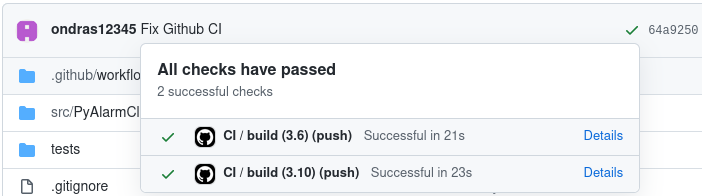
\includegraphics[width=0.90\textwidth]{github-CI}
    \caption{Výsledek úspěšného běhu \acs{CI} na platformě Github actions}
    \label{fig:PyAlarmClock CI}
\end{figure}
